\section{D -- Iroha and a Grid}

\begin{frame}[fragile]{Problema}

We have a large square grid with $H$ rows and $W$ columns. Iroha is now standing in the top-left
cell. She will repeat going right or down to the adjacent cell, until she reaches the bottom-right
cell.

However, she cannot enter the cells in the intersection of the bottom $A$ rows and the leftmost $B$
columns. (That is, there are $A\times B$ forbidden cells.) There is no restriction on entering the
other cells.

Find the number of ways she can travel to the bottom-right cell.

Since this number can be extremely large, print the number modulo $10^9 + 7$.

\end{frame}

\begin{frame}[fragile]{Entrada e saída}

\textbf{Constraints}

\begin{itemize}
    \item $1\leq H, W\leq 100,000$
    \item $1\leq A < H$
    \item $1\leq B < W$
\end{itemize}

\vspace{0.1in}

\textbf{Input}

Input is given from Standard Input in the following format:
\begin{atcoderio}{llll}
$H$ & $W$ & $A$ & $B$ \\
\end{atcoderio}

\textbf{Output}

Print the number of ways she can travel to the bottom-right cell, modulo $10^9 + 7$.

\end{frame}

\begin{frame}[fragile]{Exemplo de entradas e saídas}

\begin{minipage}[t]{0.55\textwidth}
\textbf{Entrada}
\begin{verbatim}
2 3 1 1


10 7 3 4


100000 100000 99999 99999


100000 100000 44444 55555
\end{verbatim}
\end{minipage}
\begin{minipage}[t]{0.4\textwidth}
\textbf{Saída}
\begin{verbatim}
2


3570


1


738162020
\end{verbatim}
\end{minipage}
\end{frame}

\begin{frame}[fragile]{Solução}

    \begin{itemize}
        \item Este problema é uma variação de um problema combinatório conhecido

        \item O problema consiste em determinar o número de maneiras de, a partir do ponto
            ($1, 1$), chegar ao ponto ($m$, $n$), podendo-se mover apenas uma unidade para à esquerda
                ou uma unidade para cima

            \begin{figure}
    \centering

    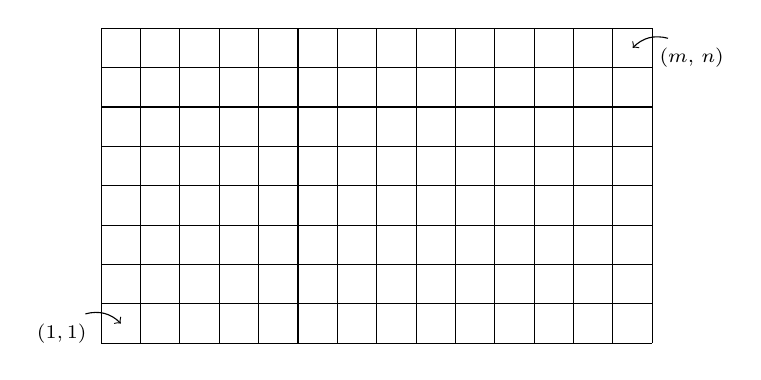
\begin{tikzpicture}[scale=0.5]
        \draw (0, 0) grid (14, 8);
        \node (A) at (-1, 0.25) { \scriptsize ($1, 1$) };
        \coordinate (B) at (0.5, 0.5);

        \node (X) at (15, 7.25) { \scriptsize ($m$, $n$) };
        \coordinate (Y) at (13.5, 7.5);

        \draw[->] (A) edge[bend left] (B);
        \draw[->] (X) edge[bend right] (Y);

    \end{tikzpicture}

\end{figure}


    \end{itemize}

\end{frame}


\begin{frame}[fragile]{Solução}

    \begin{itemize}
        \item Todos os diferentes caminhos compartilham o fato que é necessário caminhar 
            exatamente $m - 1$ passos para a direita e $n - 1$ passos para cima

        \item A diferença reside onde estes passos vão acontecer

        \item Uma vez determinado os pontos onde os passos para direita irão ocorrer, os para
            cima ficam determinados

        \item Assim, o número de maneiras distinas de se chegar a ($m, n$) a partir de ($1, 1$)
            é dado por
        \[
            ways(m, n) = \binom{(m - 1) + (n - 1)}{m - 1}
        \]
    \end{itemize}

\end{frame}

\begin{frame}[fragile]{Solução}

    \begin{itemize}
        \item A diferença entre o problema combinatório conhecido e problema atual é a região
            bloqueada

        \item Outra diferença é Iroha está no canto superior esquerdo, então é útil posicionar o 
            ponto ($1, 1$) neste ponto de partida 

            \begin{figure}
    \centering

    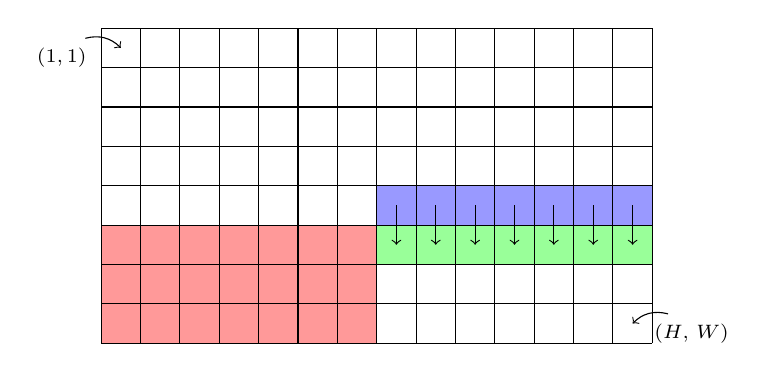
\begin{tikzpicture}[scale=0.5]

        \draw[fill=red!40] (0, 0) rectangle (7, 3);
        \draw[fill=blue!40] (7, 3) rectangle (14, 4);
        \draw[fill=green!40] (7, 2) rectangle (14, 3);

        \draw (0, 0) grid (14, 8);

        \node (A) at (-1, 7.25) { \scriptsize ($1, 1$) };
        \coordinate (B) at (0.5, 7.5);

        \node (X) at (15, 0.25) { \scriptsize ($H$, $W$) };
        \coordinate (Y) at (13.5, 0.5);

        \draw[->] (A) edge[bend left] (B);
        \draw[->] (X) edge[bend right] (Y);

        \draw[->] (7.5, 3.5) -- (7.5, 2.5);
        \draw[->] (8.5, 3.5) -- (8.5, 2.5);
        \draw[->] (9.5, 3.5) -- (9.5, 2.5);
        \draw[->] (10.5, 3.5) -- (10.5, 2.5);
        \draw[->] (11.5, 3.5) -- (11.5, 2.5);
        \draw[->] (12.5, 3.5) -- (12.5, 2.5);
        \draw[->] (13.5, 3.5) -- (13.5, 2.5);

    \end{tikzpicture}

\end{figure}


    \end{itemize}

\end{frame}

\begin{frame}[fragile]{Solução}

    \begin{itemize}
        \item Assim, os caminhos são montado em duas etapas:
        \begin{enumerate}
            \item Alcançar uma das posições à direita do bloqueio, na altura imediatamente 
                anterior (marcados em azul na figura)

            \item Após se mover para a posição imediatamente abaixo (em verde, indicado pelas
                setas), se dirigir para o pontot $(H, W)$
        \end{enumerate}

        \item Como os caminhos de cada etapa são independentes, os produtos das quantidades de
            maneiras distintas de se chegar aos pontos desejados devem ser acumulados
            na resposta

        \item Para computar os coeficientes binomiais de maneira eficiente, deve-se precomputar
            os valores dos fatoriais e seus inversos multiplicativos 
    \end{itemize}

\end{frame}

\begin{frame}[fragile]{Solução}

    \begin{itemize}
        \item Como $p = 10^9 + 7$ é primo, os inversos multiplicativos podem ser computado por
            meio do Teorema de Euler:
        \[
            a^{p - 2} \equiv \Mod{a^{-1}}{p}
        \]

        \item Este exponencial pode ser computada em $O(\log p)$, por meio de um algoritmo de 
            divisão e conquista, denominado exponenciação rápida

        \item Considere o coeficiente $\binom{n}{m}$

        \item Neste problema, o maior valor possível para $n$ é a soma $H + W$, de modo que só 
            é preciso pré-computar os fatoriais até este valor

        \item Assim a complexidade da solução é $O((H + W)\log p)$
    \end{itemize}

\end{frame}
\begin{frame}[fragile]{Solução $O((H + W)\log p)$}
    \inputsnippet{cpp}{1}{21}{codes/D.cpp}
\end{frame}

\begin{frame}[fragile]{Solução $O((H + W)\log p)$}
    \inputsnippet{cpp}{22}{42}{codes/D.cpp}
\end{frame}

\begin{frame}[fragile]{Solução $O((H + W)\log p)$}
    \inputsnippet{cpp}{43}{63}{codes/D.cpp}
\end{frame}

\begin{frame}[fragile]{Solução $O((H + W)\log p)$}
    \inputsnippet{cpp}{64}{84}{codes/D.cpp}
\end{frame}
